\documentclass[tikz,border=5mm]{standalone}
\usepackage{tikz}
\usepackage{xcolor}
\usetikzlibrary{shapes.geometric, arrows.meta, positioning, fit, backgrounds, shadows, calc}

\definecolor{coreFill}{RGB}{250, 250, 250}
\definecolor{blockFill}{RGB}{255, 255, 255}
\definecolor{lineColor}{RGB}{50, 60, 70}
\definecolor{headerText}{RGB}{0, 0, 0}
\definecolor{subText}{RGB}{80, 80, 80}
\definecolor{accentGreen}{RGB}{118, 185, 0}
\definecolor{groupBg}{RGB}{242, 245, 248}
\definecolor{borderColor}{RGB}{180, 190, 200}

\begin{document}
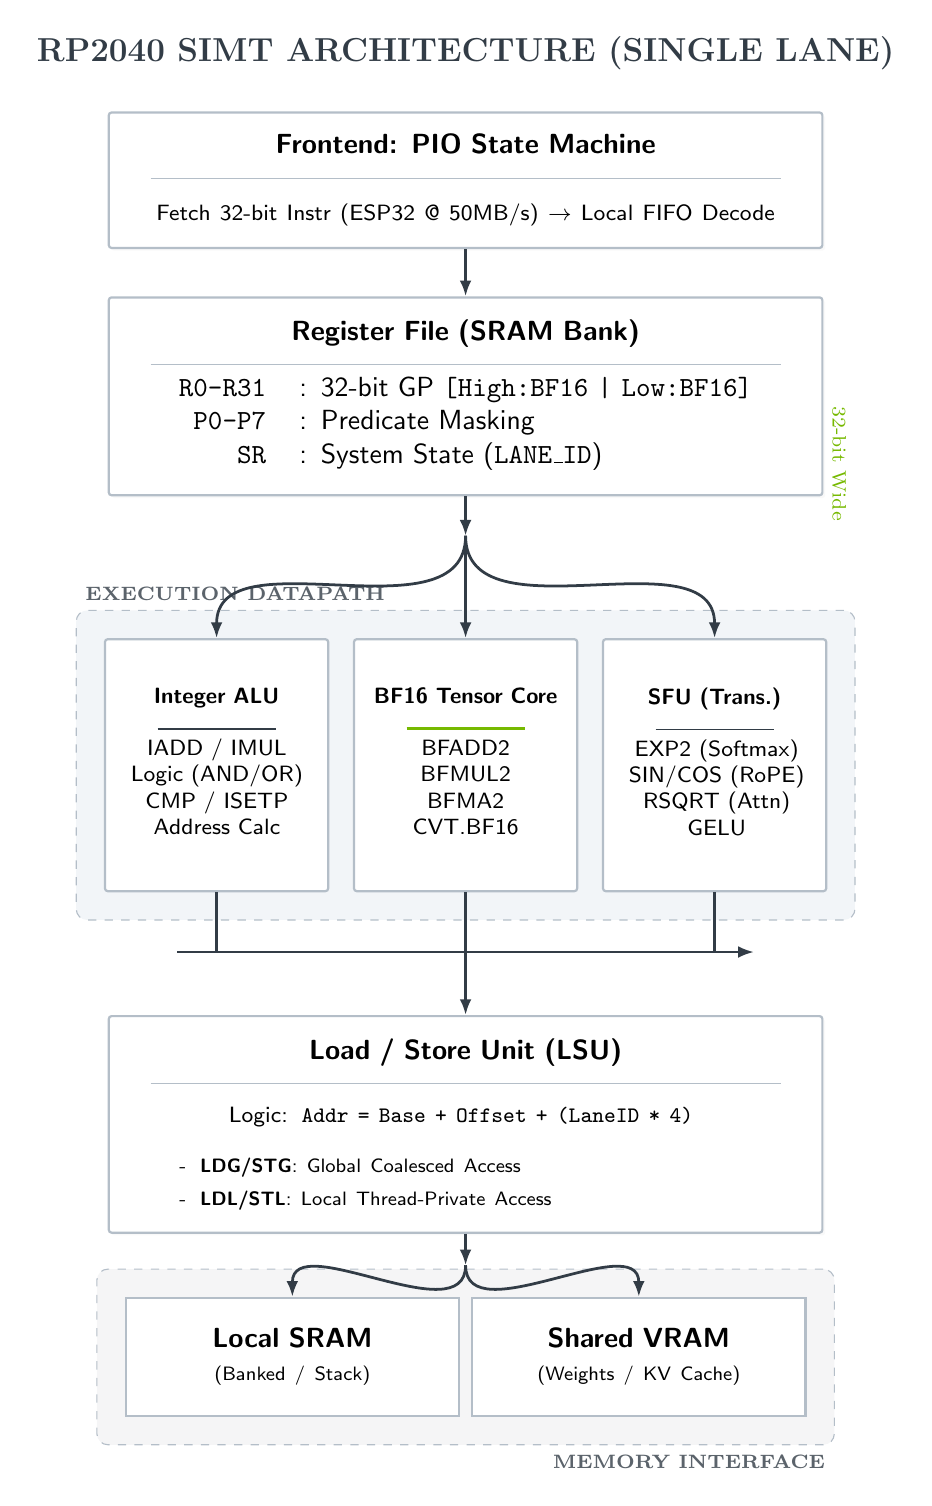
\begin{tikzpicture}[node distance=0.8cm]

% Style definitions
\tikzset{
    base/.style={
        rectangle, draw=borderColor, line width=0.8pt, font=\sffamily, align=center
    },
    module/.style={
        base, fill=blockFill, rounded corners=1pt, text width=8.5cm,
        inner sep=8pt, drop shadow={opacity=0.05, shadow xshift=1pt, shadow yshift=-1pt}
    },
    eu/.style={
        base, fill=white, text width=2.6cm, minimum height=3.2cm,
        rounded corners=1pt, font=\sffamily\footnotesize, anchor=north
    },
    labeltext/.style={font=\bfseries\small, text=headerText, align=center},
    code/.style={font=\ttfamily\footnotesize, color=subText},
    wire/.style={
        draw=lineColor, line width=1.0pt, -{Latex[length=2mm, width=1.5mm]}, rounded corners=2pt
    },
    group/.style={
        draw=borderColor, dashed, fill=groupBg, rounded corners=4pt, inner sep=10pt
    }
}

% Title
\node (top_label) [font=\bfseries\large, color=lineColor] {RP2040 SIMT ARCHITECTURE (SINGLE LANE)};

% Frontend / Fetch
\node (frontend) [module, below=0.4cm of top_label] {
    \textbf{Frontend: PIO State Machine} \\[-0.3em]
    \textcolor{borderColor}{\rule{8cm}{0.4pt}} \\[0.3em]
    {\footnotesize Fetch 32-bit Instr (ESP32 @ 50MB/s) $\rightarrow$ Local FIFO Decode}
};

% Register File
\node (regfile) [module, below=0.6cm of frontend] {
    \textbf{Register File (SRAM Bank)} \\[-0.3em]
    \textcolor{borderColor}{\rule{8cm}{0.4pt}} \\[0.2em]
    \begin{tabular}{r l}
        \textbf{\texttt{R0-R31}} & : 32-bit GP \texttt{[High:BF16 | Low:BF16]} \\
        \textbf{\texttt{P0-P7}} & : Predicate Masking \\
        \textbf{\texttt{SR}} & : System State (\texttt{LANE\_ID})
    \end{tabular}
};

% Execution Units
\node (alu_bf16) [eu, below=1.8cm of regfile] {
    \textbf{BF16 Tensor Core} \\
    \textcolor{accentGreen}{\rule{1.5cm}{1pt}} \\
    \vspace{0.2em}
    \begin{tabular}{c}
        BFADD2 \\ BFMUL2 \\ BFMA2 \\ CVT.BF16
    \end{tabular}
};

\node (alu_int) [eu, left=0.3cm of alu_bf16] {
    \textbf{Integer ALU} \\
    \textcolor{lineColor}{\rule{1.5cm}{0.5pt}} \\
    \vspace{0.2em}
    \begin{tabular}{c}
        IADD / IMUL \\ Logic (AND/OR) \\ CMP / ISETP \\ Address Calc
    \end{tabular}
};

\node (sfu) [eu, right=0.3cm of alu_bf16] {
    \textbf{SFU (Trans.)} \\
    \textcolor{lineColor}{\rule{1.5cm}{0.5pt}} \\
    \vspace{0.2em}
    \begin{tabular}{c}
        EXP2 (Softmax) \\ SIN/COS (RoPE) \\ RSQRT (Attn) \\ GELU
    \end{tabular}
};

% Execution core background
\begin{pgfonlayer}{background}
    \node (core_bg) [group, fit=(alu_int)(sfu)(alu_bf16)] {};
    \node [anchor=south west, font=\bfseries\scriptsize, color=lineColor!80] 
        at (core_bg.north west) {EXECUTION DATAPATH};
\end{pgfonlayer}

% Load / Store Unit
\node (lsu) [module, below=1.2cm of core_bg.south] {
    \textbf{Load / Store Unit (LSU)} \\[-0.3em]
    \textcolor{borderColor}{\rule{8cm}{0.4pt}} \\[0.2em]
    {\footnotesize Logic: \texttt{Addr = Base + Offset + (LaneID * 4)}}
    \vspace{0.2em}
    \begin{itemize}
         \setlength\itemsep{0em}
         \scriptsize
         \item[-] \textbf{LDG/STG}: Global Coalesced Access
         \item[-] \textbf{LDL/STL}: Local Thread-Private Access
    \end{itemize}
};

% Memory Hierarchy
\node (mem_sram) [base, fill=white, below=0.8cm of lsu, text width=4cm, xshift=-2.2cm, minimum height=1.5cm] {
    \textbf{Local SRAM} \\
    \scriptsize (Banked / Stack)
};

\node (mem_vram) [base,fill=white, below=0.8cm of lsu, text width=4cm, xshift=2.2cm, minimum height=1.5cm] {
    \textbf{Shared VRAM} \\
    \scriptsize (Weights / KV Cache)
};

\begin{pgfonlayer}{background}
    \node (mem_bg) [group, fit=(mem_sram)(mem_vram), fill=lineColor!5] {};
    \node [anchor=north east, font=\bfseries\scriptsize, color=lineColor!80] 
        at (mem_bg.south east) {MEMORY INTERFACE};
\end{pgfonlayer}

% Connections
\draw [wire] (frontend) -- (regfile);

\coordinate (dispatch_point) at ($(regfile.south) + (0,-0.5)$);
\draw [wire] (regfile.south) -- (dispatch_point);
\draw [wire] (dispatch_point) to[out=-90, in=90] (alu_int.north);
\draw [wire] (dispatch_point) -- (alu_bf16.north);
\draw [wire] (dispatch_point) to[out=-90, in=90] (sfu.north);

\coordinate (collect_y) at ($(core_bg.south) + (0,-0.4)$);

% All arrows point straight down
\draw [line width=1.0pt, draw=lineColor] (alu_int.south) -- (alu_int.south |- collect_y);
\draw [line width=1.0pt, draw=lineColor] (alu_bf16.south) -- (alu_bf16.south |- collect_y);
\draw [line width=1.0pt, draw=lineColor] (sfu.south) -- (sfu.south |- collect_y);

% Horizontal collection bus
\draw [wire] ($(alu_int.south |- collect_y) + (-0.5,0)$) -- ($(sfu.south |- collect_y) + (0.5,0)$);
% Center arrow down to LSU
\draw [wire] ($(alu_bf16.south |- collect_y)$) -- (lsu.north);

\coordinate (mem_split) at ($(lsu.south) + (0,-0.4)$);
\draw [wire] (lsu.south) -- (mem_split);
\draw [wire] (mem_split) to[out=-90, in=90] (mem_sram.north);
\draw [wire] (mem_split) to[out=-90, in=90] (mem_vram.north);

\node [right=0.2cm of regfile, font=\scriptsize, color=accentGreen, rotate=-90] {32-bit Wide};

\end{tikzpicture}
\end{document}
